\section{Numerical experiments}
\label{sec-4}

\begin{comment}
\textit{
\begin{itemize}
    \item Description of how the bounds have been integrated in ChASE together with an automatic mechanism of algorithm selection
    \item experiments comparing the bound from above of the condition number for several system and increasing iteration number (similar to ChASE-cholQR manuscript)
    \item experiments comparing performance gains obtained using bound estimates to switch to progressively less ill-conditioned array of vectors as the ChASE iteration index increases 
\end{itemize}
}
\end{comment}

The numerical behavior and the benchmark of ChASE has been performed on the cluster JURECA-DC  at J\"ulich Supercomputing Centre in Germany, which has 480 standard homogeneous compute nodes. Each node is equipped two 64 cores AMD EPYC 7742 CPUs @ 2.25 GHz ($16 \times 32$ GB DDR4 Memory), and the interconnects are InfiniBand HDR100 Mellanox Connect-X6. ChASE has been compiled with the default software stack on JURECA-DC.
The C/C++ compiler is GCC 13.3.0, the MPI library is OpenMPI 5.0.5, and the BLAS/LAPACK libraries are Intel MKL 2024.2.0. 

For the tests on JURECA-DC, the number of MPI ranks per node and OpenMP threads per rank are respectively $4$ and $32$. The threshold tolerance for residuals {\tt tol} is fixed as $10^{-10}$, and the degree optimization of ChASE filter is always enabled unless otherwise specified. All tests in this paper are performed in double-precision.

\subsection{Parallel Scheme in ChASE}

ChASE employs a hybrid parallelization strategy tailored to efficiently handle large-scale eigenproblems on distributed-memory systems. The Chebyshev filter is applied on a 2D MPI process grid, with the number of processes chosen to form a nearly square grid whenever possible, which is preferred to balance communication and computation. The filtering procedure exploits the Hermitian or symmetric structure of the target matrix to optimize the matrix–matrix multiplication kernel. Depending on the polynomial degree of the filter, this operation may involve collective allreduce operations either along the row or column communicators of the 2D grid.

The QR factorization within ChASE, in contrast, is performed on a 1D column communicator derived from the 2D grid. Each column communicator contains a subset of MPI processes corresponding to a vertical partition of the matrix. Within each communicator, the QR factorization is executed in parallel, while the resulting factorization is redundant across different column communicators. %This design reduces communication overhead and allows the QR to scale independently of the global 2D grid size.

Such a separation of parallelism---2D for filtering, 1D for QR---ensures that both the computationally dominant filter and the numerically critical QR factorization achieve high efficiency. The chosen scheme also naturally accommodates the optimized filter profile based on the matrix structure. For further details on the parallel design, implementation choices, and the reasoning behind the column-redundant QR, we refer the reader to \cite{Wu2022chase}.

\subsection{Test Matrix Suite: DFT and BSE matrices}

For the numerical test and benchmarks, we make use of a collection of eigenproblems coming from domain applications. Essential details of these problems are listed in Table \ref{tab:real_world matrix}, including a short acronym, the size, the number of eigenpairs sought after, the size of extra searching space used in ChASE, the application software used to extract them, the type of each problem, \nev--the number of eigenparis to compute required from real world applications, and \nex--the size of external searching space.

The \text{FLEUR} problems are generated by the FLEUR code \cite{wortmann2023fleur}, which implements a full-potential linearized augmented plane wave (FLAPW) all-electron method. In this approach, the wavefunctions are expanded using augmented plane waves inside muffin-tin spheres and plane waves in the interstitial region, leading to a highly accurate but computationally intensive basis set. In contrast, the FHI-aims DFT calculations \cite{blum2009ab} employ numeric atom-centered orbitals (NAOs) as basis functions, which are strictly localized around atoms and enable efficient evaluation of integrals. This results in Hamiltonian and overlap matrices with different spectral properties compared to FLAPW-based FLEUR matrices. Specifically, FHI-aims matrices tend to have smaller bandwidth and more clustered eigenvalues due to the local nature of the orbitals, whereas FLEUR matrices are typically denser and have more evenly distributed eigenvalues across the spectrum.

The BSE UIUC problems are obtained from a fork of the Jena BSE code developed at the University of Illinois Urbana-Champaign \cite{zhang2021solving}, which builds on the underlying DFT Hamiltonians to compute electron-hole excitations. These problems typically exhibit a clustered spectrum of eigenvalues corresponding to low-energy excitations, which poses distinct challenges for iterative eigenvalue solvers.

By including eigenproblems from DFT calculations coming two distinct application codes using different discretization schemes, as well as from BSE simulations, the test suite  covers a range of spectral characteristics, matrix sizes, and numerical complexities, providing a comprehensive benchmark for evaluating the performance and robustness of ChASE. As the spectra of matrices from FHI-aims and Jena BSE is typically denser and more clustered, it requires a relatively larger searching space \nex compared to the corresponding \nev (see Table \ref{tab:real_world matrix}).

\subsection{Exact Condition number vs estimated}

In this section, we illustrate the effectiveness of the upper bounds introduced in Section \ref{sec-3} for the condition number of the rectangular matrix filtered by the Chebyshev filter\footnote{If some eigenpairs are locked, this should be the union of the locked eigenvectors and the filtered unconverged ones}. The test problems considered here are the ones listed in Table \ref{tab:real_world matrix}. The results are shown in Fig. \ref{fig:condEst-all}, which compare the estimated condition number $\cdest$ against an accurate computation of the condition number $\cd$ of the filtered matrices at each iteration of ChASE until convergence.

We performed the tests on the JURECA-DC cluster, using 4 nodes. All tests were carried out either with the Chebyshev polynomial degree optimization enabled ({\it opt}) or disabled ({\it no-opt}) to highlight how the condition number estimation depends on the optimization mechanism. For {\it no-opt}, the Chebyshev polynomial degree is fixed to $20$ at every iteration. For {\it opt}, the initial degree is $20$ for the first iteration and is dynamically adjusted at later iterations for each filtered vector with a maximal degree capped at $36$ to prevent excessive ill-conditioning.

As already defined in the previous sections, given a rectangular matrix $M$ its condition number $\cd$ is equal to $\frac{\sigma_{max}(M)}{\sigma_{min}(M)}$.  where $\sigma_{max}(M)$ and $\sigma_{min}(M)$ represent the maximal and minimal singular values of $M$. For this test, the matrix $M$ is distributed along the column communicator, and its singular values are computed directly via ScaLAPACK parallel SVD routines, specifically {\sf PDGESVD} and {\sf PZGESVD} for the real and complex double-precision cases, respectively. The estimated condition number $\cdest$ is given, in its most general form by Eq.~\eqref{eq:full-est}, which reduces to $\rto {k+1}{m}$ when the degree optimization is disabled ({\it no-opt}). The case without deflation and locking (Eq.~\ref{eq:simple-est}) is automatically recovered at the very first 1-2 iterations when no eigenpair has yet converged.

\begin{table}[t]
\footnotesize
	\renewcommand{\arraystretch}{1.3}
	\caption{List of DFT matrices for numerical tests.}\label{tab:real_world matrix}
	\centering
	\begin{tabular}{C{2.5cm}|cccC{2.cm}C{2.cm} c}
		\toprule
  Name & $N$ & {\nev} & {\nex} & Problem Type&Code Source & Type \\
  \midrule
  \textsc{NaCl 9k}   & 9273 & 256 & 60 & DFT &\textbf{FLEUR} & Hermitian \\
  \hline
  \textsc{AuAg 13k}   & 13379 & 972 & 100 & DFT&\textbf{FLEUR} & Hermitian\\
  \hline  
  \textsc{TiO2 12k}   & 12455 & 1076 & 100 &DFT &\textbf{FLEUR} & Hermitian\\
  \hline  
  \textsc{TiO2 29k}   & 29528 & 2560 & 400 & DFT&\textbf{FLEUR} & Hermitian\\
  \hline  
  \textsc{HfO2 62k}    & 62681 & 100 & 100 & BSE&\textbf{BSE UIUC}& Hermitian \\  
  \hline  
  \textsc{In2O3 76k}  & 76887 & 120 & 60 & BSE&\textbf{BSE UIUC}& Hermitian\\
  \hline
  \textsc{In2O3 115k}  & 115459 & 2400 & 1600 & BSE &\textbf{BSE UIUC}& Hermitian \\
  \hline  
  \textsc{Si Graphene 50k}    & 51476 & 2400 & 1600 & DFT&\textbf{FHI-aims} & Symmetric\\
  \hline  
  \textsc{Cu$_2$BaSnS$_4$ 80k}    & 80250 & 3600 & 2400 & DFT&\textbf{FHI-aims} & Symmetric\\  
		\bottomrule
	\end{tabular}
\end{table}

\begin{figure}[htbp]
\centering

% Row 1
\condEstSubplot{NaCl-9k}{(a) NaCl 9k}
\hfill
\condEstSubplot{AuAg-13k}{(b) AuAg 13k}
\hfill
\condEstSubplot{TiO2-12k}{(c) TiO$_2$ 12k}
\vspace{0.8em}
% Row 2
\condEstSubplot{TiO2-29k}{(d) TiO$_2$ 29k}
\hfill
\condEstSubplot{HfO2-62k}{(e) HfO2 62k}
\hfill
\condEstSubplot{In2O3-76k}{(f) In$_2$O$_3$ 76k}

\vspace{0.8em}
% Row 3
\condEstSubplot{In2O3-115k}{(g) In$_2$O$_3$ 115k}
\hfill
\condEstSubplot{SiC_graphene_50k}{(h) SiC graphene 50k}
\hfill
\condEstSubplot{Cu2BaSnS4_80k}{(i) Cu$_2$BaSnS$_4$ 80k}

\vspace{1em}

% Unified legend
\begin{center}
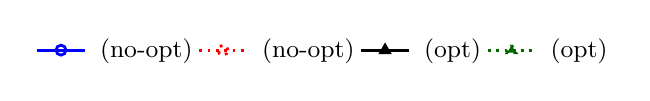
\begin{tikzpicture}
\begin{axis}[
    width=0.8\linewidth,
    height=2cm,
    hide axis,
    xmin=0, xmax=1,
    ymin=0, ymax=1,
    clip=true,
    legend columns=4,
    legend style={
        draw=none,
        font=\small,
        at={(0.5,0.5)},
        anchor=center,
        fill=none,
        cells={anchor=west},
    },
    every axis plot/.append style={opacity=0},
    legend image post style={opacity=1},
]
% Create invisible plots for legend entries only
\addplot[mark=o, solid, line width=1pt, mark size=1.8pt, color=blue] coordinates {(0.5,0.5) (0.6,0.6)};
\addlegendentry{$\cd$ (no-opt)}
\addplot[mark=o, dotted, line width=1pt, mark size=1.8pt, color=red] coordinates {(0.5,0.5) (0.6,0.6)};
\addlegendentry{$\cdest$ (no-opt)}
\addplot[mark=triangle*, solid, line width=1pt, mark size=1.8pt, color=black] coordinates {(0.5,0.5) (0.6,0.6)};
\addlegendentry{$\cd$ (opt)}
\addplot[mark=triangle*, dotted, line width=1pt, mark size=1.8pt, color=green!40!black] coordinates {(0.5,0.5) (0.6,0.6)};
\addlegendentry{$\cdest$ (opt)}
\end{axis}
\end{tikzpicture}
\end{center}


\vspace{0.5em}
\caption{Condition estimates per iteration for various materials with and without optimization. 
Subplots (a)--(i) show results for different material systems.}
\label{fig:condEst-all}
\end{figure}

Fig. \ref{fig:condEst-all} shows that the estimated condition number, with and without degree optimization, always bounds from above the computed condition number, making it an effective and reliable estimate. For many cases, the ratio between the $\cdest$ and $\cd$ is always below $2$. For some cases (e.g., {\it opt} case for AuAg 13k or TiO$_2$ 12k), this ratio can be larger than $\mathcal{O}(10^4)$ for a few initial iterations, where no eigenpairs have been locked yet. This may be caused by the facts that the estimates for the parameters $e$ and $c$ provided by ChASE could be quite inaccurate for the first 2 to 3 iterations. Independently from its strictness, $\cdest$ always bound $\cd$ from above and so it constitutes a reliable parameter for ChASE to switch from a more stable QR factorization, such as $s$-Cholesky QR factorization, to the less stable but more efficient CholeksyQR2, even CholeskyQR1 in the last one or two iterations where the estimations are $\mathcal{O}(1)$. 

In the {\it no-opt} case, the highest condition number comes at the first iteration. To clarify, in Fig. \ref{fig:condEst-all}, step $0$ corresponds to the QR factorization of the randomly generated initial guess vectors, occurring before the first application of the Chebyshev filter. Therefore, if the condition number of $M$ at the first iteration is below a certain threshold, the $s$-CholeskyQR2 can be avoided in any of the following iterations. Conversely, in the {\it opt} case the condition number of $M$ at the early stage can be much larger than the one at the first iteration. This effect is caused by the higher maximal degree allowed during the degree optimization procedure and it is controllable by the user by setting a relative smaller maximal degree for the degree optimization. Observe, though, that ChASE with degree optimization can always converge considerably faster than ChASE without degree optimization (e.g., In$_2$O$_3$ 115k). In conclusion, our upper bound estimation of the condition number for the filtered matrix ensure that the proposed heuristic to switch between QR variants is reliable throughout the entire execution cycle of ChASE. 

\subsection{ChASE with CholeskyQR vs Householder QR}

In this section, we compare the numerical behavior of ChASE using either a Householder QR (HHQR) factorization at every iteration or the automatic selection of QR variants based on the heuristic introduced in Section \ref{sec:Replacing Householder QR with Communication-Avoiding CholeskyQR Variants}. Here, HHQR refers to the Householder QR implementation provided by ScaLAPACK, executed on a 1D MPI grid independently over each column communicator. The block size for the ScaLAPACK block-cyclic distribution is set to $64$. All tests in this section were run on $4$ nodes of the JURECA-DC cluster, using all available CPU cores. Each reported value corresponds to the average of $5$ repetitions.

The test problems are those listed in Table \ref{tab:real_world matrix}. In all cases, the matrix to be factorized has dimensions $N\times(\nev+\nex)$. Tables \ref{table:hh_vs_chol_cpu} reports the total number of matrix-vector multiplications (MatVecs)\footnote{At each ChASE iteration, the Chebyshev filter is applied to a rectangular matrix $M$ where each column may use a different polynomial degree. The number of matrix-vector multiplications (MatVecs) is accumulated over all unconverged eigenvectors and all iterations, providing a measure of the computational work in the filter and offering insight into the convergence behavior of individual filtered vectors.}
, the number of ChASE iterations to convergence, the total time-to-solution, and the time spent in the QR factorization.
\begin{table}[t]
\footnotesize
\renewcommand{\arraystretch}{1.3}
\caption{Comparison of ChASE-CPU with HHQR and CholeksyQR}\label{table:hh_vs_chol_cpu}
\centering
\begin{tabular}{C{2.5cm}|C{1.8cm}|C{1.2cm}C{1.4cm}C{1.1cm}C{1.8cm}}
\toprule
Type                     & QR Impl.   & MatVecs & Iters. & All (s) & QR (s) \\ \midrule
\multirow{2}{*}{\textsc{NaCl 9k}}
                         & HHQR   & 34,206 & 6 & 8.64 & 1.34  \\ 
                         & CholeskyQR  & 34,212 & 6 & 8.14 & 0.51 \\ \hline
\multirow{2}{*}{\textsc{AuAg 13k}}
                         & HHQR   & 106,542 & 8 & 40.13 & 8.72 \\ 
                         & CholeskyQR & 106,618  & 8 & 32.96 & 1.72  \\ \hline
\multirow{2}{*}{\textsc{TiO2 12k}}
                         & HHQR   & 94,724 & 6 & 32.47 & 7.62 \\ 
                         & CholeskyQR & 93,904 & 6 & 26.05 & 1.92  \\ \hline  
\multirow{2}{*}{\textsc{TiO2 29k}}
                         & HHQR   & 212,024 & 5 & 323.21 & 81.56 \\ 
                         & CholeskyQR & 211,984 & 5 & 278.11 & 16.23 \\  \hline 
\multirow{2}{*}{\textsc{HfO2 62k}}
                         & HHQR   & 19,614 & 5 & 201.41 & 5.91 \\ 
                         & CholeskyQR & 19,614 & 5 & 195.33 & 1.95 \\ \hline                             
\multirow{2}{*}{\textsc{In2O3 76k}}
                         & HHQR   & 15,980 & 5 & 284.62 & 6.97 \\  
                         & CholeskyQR & 15,976 & 5 & 278.25 & 1.81 \\  \hline 
\multirow{2}{*}{\textsc{In2O3 115k}}
                         & HHQR   & 229,714 & 3 & 2533.05 & 184.65 \\ 
                         & CholeskyQR & 229,716 & 3 & 2439.24 & 74.91 \\    \hline                        
\multirow{2}{*}{\textsc{Si Graphene 50k}}
                         & HHQR   & 240,554 & 3 & 263.33 & 53.98 \\ 
                         & CholeskyQR & 240,536 & 3 & 208.91 & 8.90 \\  \hline   
\multirow{2}{*}{\textsc{Cu$_2$BaSnS$_4$ 80k}}
                         & HHQR   & 413,084 & 4 & 911.62 & 139.72 \\ 
                         & CholeskyQR & 429,620 & 4 & 747.72 & 30.11 \\                         
\bottomrule
\end{tabular}
\label{tab:chol_vs_hh_cpu}
\end{table}
The results show that ChASE equipped with CholeskyQR achieves numerically identical convergence compared to HHQR: the number of iterations and MatVec operations remain effectively the same for all test problems. The main difference is in performance: CholeskyQR consistently reduces the time spent in QR factorizations, with speedups ranging from $2$-$5\times$ for moderate problem sizes ($\nev\lesssim1000$) and up to $4$-$6\times$ for larger problems ($\nev\gtrsim2000$), leading to a total time-to-solution reduction of 10–20\% depending on the problem.

In conclusion, these results confirm that replacing a stable HHQR with CholeskyQR, guided by the condition number bounds introduced in Section \ref{sec-3}, preserves the numerical behavior of ChASE while providing substantial computational reduction, particularly for problems with a larger number of desired eigenpairs. Detailed parallel scaling and performance analysis are discussed in the following section.

\subsection{Strong scaling}

We evaluate the strong scaling behavior of ChASE using In$_2$O$_3$ 115k eigenproblem defined in Table \ref{tab:real_world matrix} with three eigenpair configurations: 1) {\bf Small} ($\nev=1200$, $\nex=600$); 2) {\bf Medium}  ($\nev=2400$, $\nex=1200$);  3) {\bf Large}  ($\nev=3600$, $\nex=2400$). These labels are used consistently throughout the section to distinguish problem sizes. All runs were performed on the JURECA-DC cluster, scaling from 16 up to 100 compute nodes with $4$ MPI ranks per node, and $32$ OpenMP threads per MPI process. The number of nodes in each benchmark is chosen to form a square MPI process grid in ChASE, which is generally preferred for performance.

Figure \ref{fig:combined_strong_scaling} reports both the total time-to-solution and parallel efficiency, along with the time and efficiency specifically for the QR factorization using CholeskyQR and Householder QR.
In ChASE, QR is performed only within the column communicator—that is, a subset of the global 2D MPI grid. For instance, in a run employing 64 nodes with 256 MPI processes in total, the column communicator typically spans only 16 MPI processes; hence, the QR timing and efficiency reflect the scaling behavior of this smaller communicator.

%\commnt{Edo}{I am not happy with the fact that the Time plots for "All" are in semilog scale while the one for "QR" are in linear scale. Can you please try to use log scale on the vertical axis and linear scale of the horizontal one? Alternatively, we can plot speedups instead of time to solution. Also change to linear scale for the horizontal axis in the "All" efficiency.}
%\commnt{XZ}{Actually, both plot used only linear scaled. Now I updated them to be y-axis with log, and x-axis with linear scale.}

%%%%%%%%%
%%%%%%%%%%
%%%%%%%%%%%
%%%%%%%%%%%%
%%%%%%%%%%%%%

\begin{figure}[t]
\centering

% ----------------- Top row -----------------
\begin{minipage}{0.3\linewidth}
\centering
\pgfplotsset{set layers}
\begin{tikzpicture}
\begin{axis}[
    width=\linewidth,
    height=1.2\linewidth,
    xlabel={Number of MPI ranks},
    ylabel={Time (s)},
    ymode=log,
    xmode=log,
    xtick={16,36,64,100},
    % ----- FORCE TICKS -----
    xtick={16,36,64,100},
    xticklabels={64,144,256,400},
    ytick={100,200,400,800},
    yticklabels={100,200,400,800},  
    scaled x ticks=false,
    scaled y ticks=false,
    title={All: Time},
    tick label style={font=\small},
    label style={font=\small},
    axis line style={black, line width=1pt},
    grid=major,
    grid style={dashed, gray!30},
    line width=1pt
]
    \addplot+[mark=o, solid, mark size=2pt, blue] coordinates {(16,530) (36,255) (64,174) (100,117.5)};
    \addplot+[mark=o, dashed, mark size=2pt, blue] coordinates {(16,570.9) (36,288.1) (64,215.2) (100,147.8)};
    % Upper CI curve
    \addplot[
        name path=upper,
        draw=none
    ] coordinates {
        (16,534) (36,258) (64,177) (100,124)
    };

    % Lower CI curve
    \addplot[
        name path=lower,
        draw=none
    ] coordinates {
        (16,526) (36,252) (64,171) (100,110)
    };

    % Confidence band
    \addplot[
        blue!20
    ] fill between[
        of= lower and upper,
    ];
    
    \addplot[
        name path=upper2,
        draw=none
    ] coordinates {
        (16,579) (36,294) (64,210) (100,152)
    };

    % Lower CI curve
    \addplot[
        name path=lower2,
        draw=none
    ] coordinates {
        (16,561) (36,282) (64,220) (100,143)
    };

    % Confidence band
    \addplot[
        blue!20
    ] fill between[
        of=lower2 and upper2,
    ];
    
% Ideal case line
\addplot[
    black,
    dash dot,
    no markers,
    line width=1pt
] coordinates {
    (16,450)
    (36,200)
    (64,112.5)
    (100,72)
};
\node at (axis cs:86,70) [anchor=south east, black, font=\small] {Ideal};
\end{axis}
\end{tikzpicture}
\end{minipage}
\hfill
\begin{minipage}{0.3\linewidth}
\pgfplotsset{set layers}
\centering
\begin{tikzpicture}
\begin{axis}[
    width=\linewidth,
    height=1.2\linewidth,
    xlabel={Number of MPI ranks},
    ylabel={Time (s)},
    xmode=log,
    ymode=log,
    % ----- FORCE TICKS -----
    xtick={16,36,64,100},
    xticklabels={64,144,256,400},
    ytick={300,600,1200,2400},
    yticklabels={300,600,1200, 2400},    
    scaled x ticks=false,
    scaled y ticks=false,
    title={All: Time},
    tick label style={font=\small},
    label style={font=\small},
    grid=major,
    axis line style={black, line width=1pt},
    grid style={dashed, gray!30},
    line width=1pt
]
    % Upper CI curve
    \addplot[
        name path=upper,
        draw=none
    ] coordinates {
        (16,1145) (36,575) (64,400) (100,300)
    };

    % Lower CI curve
    \addplot[
        name path=lower,
        draw=none
    ] coordinates {
        (16,1135) (36,565) (64,380) (100,290)
    };

    % Confidence band
    \addplot[
        red!20
    ] fill between[
        of=upper and lower,
    ];
    
    \addplot[
        name path=upper2,
        draw=none
    ] coordinates {
        (16,1185) (36,640) (64,455) (100,365)
    };

    % Lower CI curve
    \addplot[
        name path=lower2,
        draw=none
    ] coordinates {
        (16,1175) (36,634) (64,439) (100,357)
    };

    % Confidence band
    \addplot[
        red!20
    ] fill between[
        of=upper2 and lower2,
    ];

    \addplot[
        name path=upper3,
        draw=none
    ] coordinates {
        (16,1900) (36,1049) (64,810) (100,703)
    };

    % Lower CI curve
    \addplot[
        name path=lower3,
        draw=none
    ] coordinates {
        (16,1880) (36,1047) (64,808) (100,701)
    };

    % Confidence band
    \addplot[
        green!20
    ] fill between[
        of=upper3 and lower3,
    ];

    \addplot[
        name path=upper4,
        draw=none
    ] coordinates {
        (16,1915) (36,1192) (64,866) (100,760)
    };

    % Lower CI curve
    \addplot[
        name path=lower4,
        draw=none
    ] coordinates {
        (16,1905) (36,1188) (64,860) (100,750)
    };

    % Confidence band
    \addplot[
        green!20
    ] fill between[
        of=upper4 and lower4,
    ];
    
%\addplot+[mark=o, solid, mark size=2pt, blue] coordinates {(16,450.9) (36,275.1) (64,151.2) (100,105.8)};
%\addplot+[mark=o, dashed, mark size=2pt, blue] coordinates {(16,487.4) (36,316.1) (64,181.1) (100,129.4)};
\addplot+[mark=square, solid, mark size=2pt, red] coordinates {(16,1140) (36,570) (64,390) (100,295)};
\addplot+[mark=square, dashed, mark size=2pt, red] coordinates {(16,1180) (36,637) (64,452) (100,361)};
\addplot+[mark=triangle, solid, mark size=2pt, green!60!black] coordinates {(16,1890) (36,1048) (64,809) (100,702)};
\addplot+[mark=triangle, dashed, mark size=2pt, green!60!black] coordinates {(16,1910) (36,1190) (64,863) (100,755)};
% Ideal case line
\addplot[
    black,
    dash dot,
    no markers,
    line width=1pt
] coordinates {
    (16,1600)
    (36,711)
    (64,400)
    (100,256)
};
\node at (axis cs:82,640) [anchor=south east, black, font=\small] {Ideal};
\end{axis}
\end{tikzpicture}
\end{minipage}
\hfill
\begin{minipage}{0.3\linewidth}
\pgfplotsset{set layers}
\centering
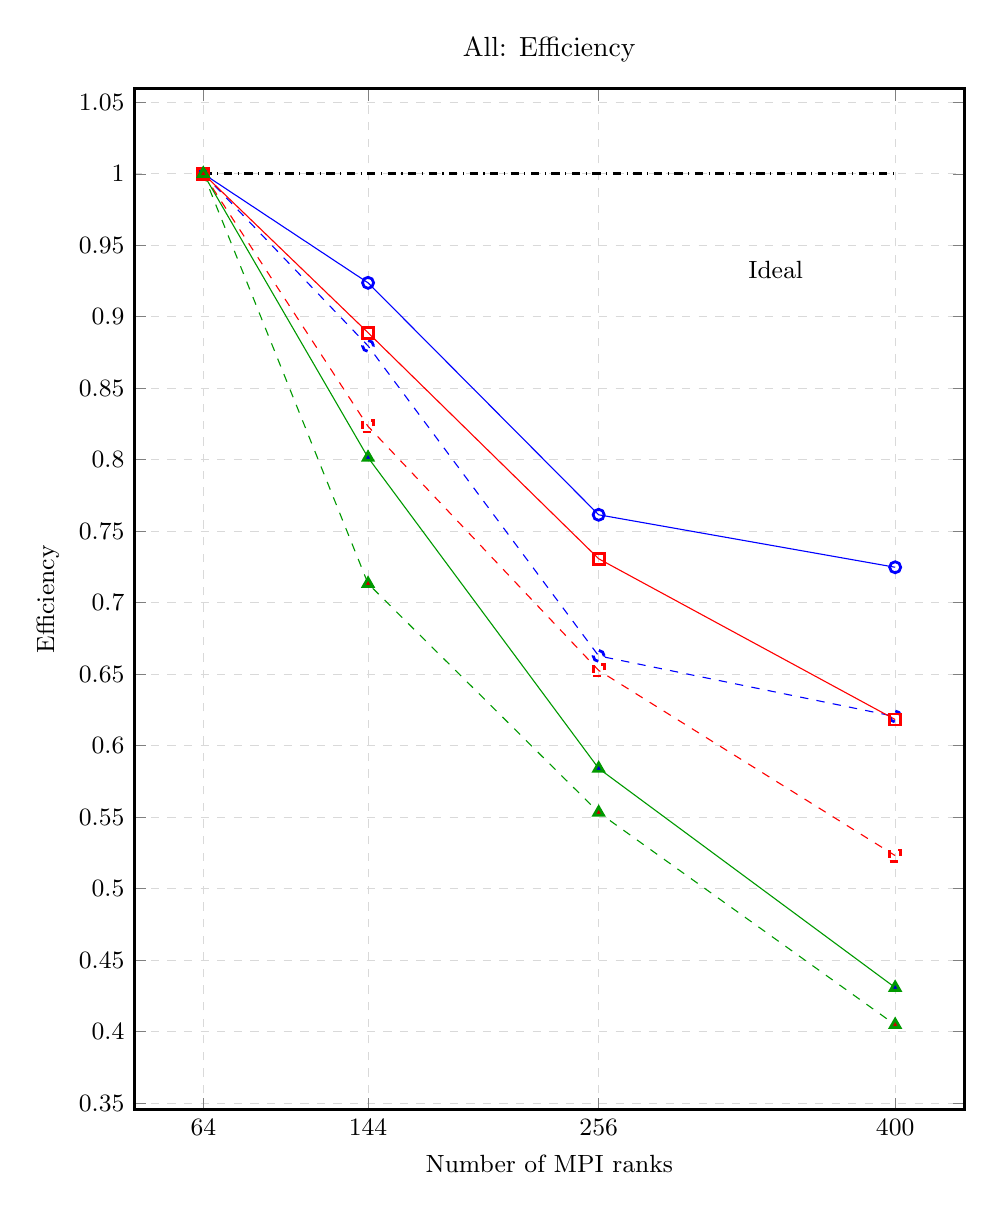
\begin{tikzpicture}
\begin{axis}[
    width=\linewidth,
    height=1.2\linewidth,
    xlabel={Number of MPI ranks},
    ylabel={Efficiency},
    xtick={16,36,64,100},
    xticklabels={64,144,256,400},
    title={All: Efficiency},
    tick label style={font=\small},
    label style={font=\small},
    grid=major,
    axis line style={black, line width=1pt},
    grid style={dashed, gray!30},
    line width=1pt
]

\addplot+[mark=o, solid, mark size=2pt, blue] coordinates {(16,1.0000) (36,530*16/255/36) (64,530*16/174/64) (100,530*16/117/100)};
\addplot+[mark=o, dashed, mark size=2pt, blue] coordinates {(16,1.0000) (36,570*16/288/36) (64,570*16/215/64) (100,570*16/147/100)};
\addplot+[mark=square, solid, mark size=2pt, red] coordinates {(16,1.0000) (36,1140*16/570/36) (64,1140*16/390/64) (100,1140*16/295/100)};
\addplot+[mark=square, dashed, mark size=2pt, red] coordinates {(16,1.0000) (36,1180*16/637/36) (64,1180*16/452/64) (100,1180*16/361/100)};
\addplot+[mark=triangle*, solid, mark size=2pt, green!60!black] coordinates {(16,1.0000) (36,1890*16/1048/36) (64,1890*16/809/64) (100,1890*16/702/100)};
\addplot+[mark=triangle*, dashed, mark size=2pt, green!60!black] coordinates {(16,1.0000) (36,1910*16/1190/36) (64,1910*16/863/64) (100,1910*16/755/100)};
\addplot[
    black,
    dash dot,
    no markers,
    line width=1pt
] coordinates {
    (16,1)
    (36,1)
    (64,1)
    (100,1)
};
\node at (axis cs:90,0.92) [anchor=south east, black, font=\small] {Ideal};
\end{axis}
\end{tikzpicture}
\end{minipage}

\vspace{1em}

% ----------------- Bottom row -----------------
\begin{minipage}{0.3\linewidth}
\pgfplotsset{set layers}
\centering
\begin{tikzpicture}
\begin{axis}[
    width=\linewidth,
    height=1.2\linewidth,
    xlabel={Number of MPI ranks},
    ylabel={Time (s)},
    ymode=log,
    xmode=log,
    xtick={4,6,8,10},
    xticklabels={8,12,16,20},
    ytick={5,10,20,40},
    yticklabels={5,10,20,40},      
    title={QR: Time},
    tick label style={font=\small},
    label style={font=\small},
    grid=major,
    axis line style={black, line width=1pt},
    grid style={dashed, gray!30},
    line width=1pt
]
\addplot+[mark=o, solid, mark size=2pt, blue] coordinates {(4,19) (6,14) (8,11.2) (10,9.2)};
\addplot+[mark=o, dashed, mark size=2pt, blue] coordinates {(4,53) (6,43) (8,41) (10,38)};

    % Upper CI curve
    \addplot[
        name path=upper,
        draw=none
    ] coordinates {
        (4,22) (6,14.5) (8,12) (10,9.5)
    };

    % Lower CI curve
    \addplot[
        name path=lower,
        draw=none
    ] coordinates {
        (4,16) (6,13.5) (8,10) (10,8.9)
    };

    % Confidence band
    \addplot[
        blue!20
    ] fill between[
        of= lower and upper,
    ];
    
    \addplot[
        name path=upper2,
        draw=none
    ] coordinates {
        (4,56) (6,46) (8,43) (10,40)
    };

    % Lower CI curve
    \addplot[
        name path=lower2,
        draw=none
    ] coordinates {
        (4,50) (6,40) (8,38) (10,36)
    };

    % Confidence band
    \addplot[
        blue!20
    ] fill between[
        of=lower2 and upper2,
    ];
    
\addplot[
    black,
    dash dot,
    no markers,
    line width=1pt
] coordinates {
    (4,33)
    (6,22)
    (8,16.5)
    (10,13.2)
};
\node at (axis cs:9.9,18) [anchor=south east, black, font=\small] {Ideal};
\end{axis}
\end{tikzpicture}
\end{minipage}
\hfill
\begin{minipage}{0.3\linewidth}
\pgfplotsset{set layers}
\centering
\begin{tikzpicture}
\begin{axis}[
    width=\linewidth,
    height=1.2\linewidth,
    xlabel={Number of MPI ranks},
    ylabel={Time (s)},
    ymode=log,
    xmode=log,
    xtick={4,6,8,10},
    xticklabels={8,12,16,20},
    ytick={20,40,80,160},
    yticklabels={20,40,80,160},  
    title={QR: Time},
    tick label style={font=\small},
    label style={font=\small},
    grid=major,
    axis line style={black, line width=1pt},
    grid style={dashed, gray!30},
    line width=1pt
]
\addplot+[mark=square, solid, mark size=2pt, red] coordinates {(4,75) (6,57) (8,46) (10,36)};
\addplot+[mark=square, dashed, mark size=2pt, red] coordinates {(4,127) (6,103) (8,91.8) (10,86.3)};
\addplot+[mark=triangle, solid, mark size=2pt, green!60!black] coordinates {(4,198) (6,150) (8,124) (10,100)};
\addplot+[mark=triangle, dashed, mark size=2pt, green!60!black] coordinates {(4,223) (6,178) (8,156) (10,146)};

    % Upper CI curve
    \addplot[
        name path=upper,
        draw=none
    ] coordinates {
        (4,78) (6,59) (8,48) (10,37)
    };

    % Lower CI curve
    \addplot[
        name path=lower,
        draw=none
    ] coordinates {
        (4,72) (6,55) (8,44) (10,35)
    };

    % Confidence band
    \addplot[
        red!20
    ] fill between[
        of=upper and lower,
    ];
    
    \addplot[
        name path=upper2,
        draw=none
    ] coordinates {
        (4,127) (6,103) (8,92) (10,87)
    };

    % Lower CI curve
    \addplot[
        name path=lower2,
        draw=none
    ] coordinates {
        (4,127) (6,103) (8,91.6) (10,85.6)
    };

    % Confidence band
    \addplot[
        red!20
    ] fill between[
        of=upper2 and lower2,
    ];

    \addplot[
        name path=upper3,
        draw=none
    ] coordinates {
        (4,200) (6,155) (8,126) (10,102)
    };

    % Lower CI curve
    \addplot[
        name path=lower3,
        draw=none
    ] coordinates {
        (4,196) (6,145) (8,122) (10,98)
    };

    % Confidence band
    \addplot[
        green!20
    ] fill between[
        of=upper3 and lower3,
    ];

    \addplot[
        name path=upper4,
        draw=none
    ] coordinates {
        (4,223) (6,179) (8,157) (10,146)
    };

    % Lower CI curve
    \addplot[
        name path=lower4,
        draw=none
    ] coordinates {
        (4,223) (6,177) (8,155) (10,146)
    };

    % Confidence band
    \addplot[
        green!20
    ] fill between[
        of=upper4 and lower4,
    ];
    
\addplot[
    black,
    dash dot,
    no markers,
    line width=1pt
] coordinates {
    (4,120)
    (6,80)
    (8,60)
    (10,48)
};
\node at (axis cs:9.9,40) [anchor=south east, black, font=\small] {Ideal};
\end{axis}
\end{tikzpicture}
\end{minipage}
\hfill
\begin{minipage}{0.3\linewidth}
\centering
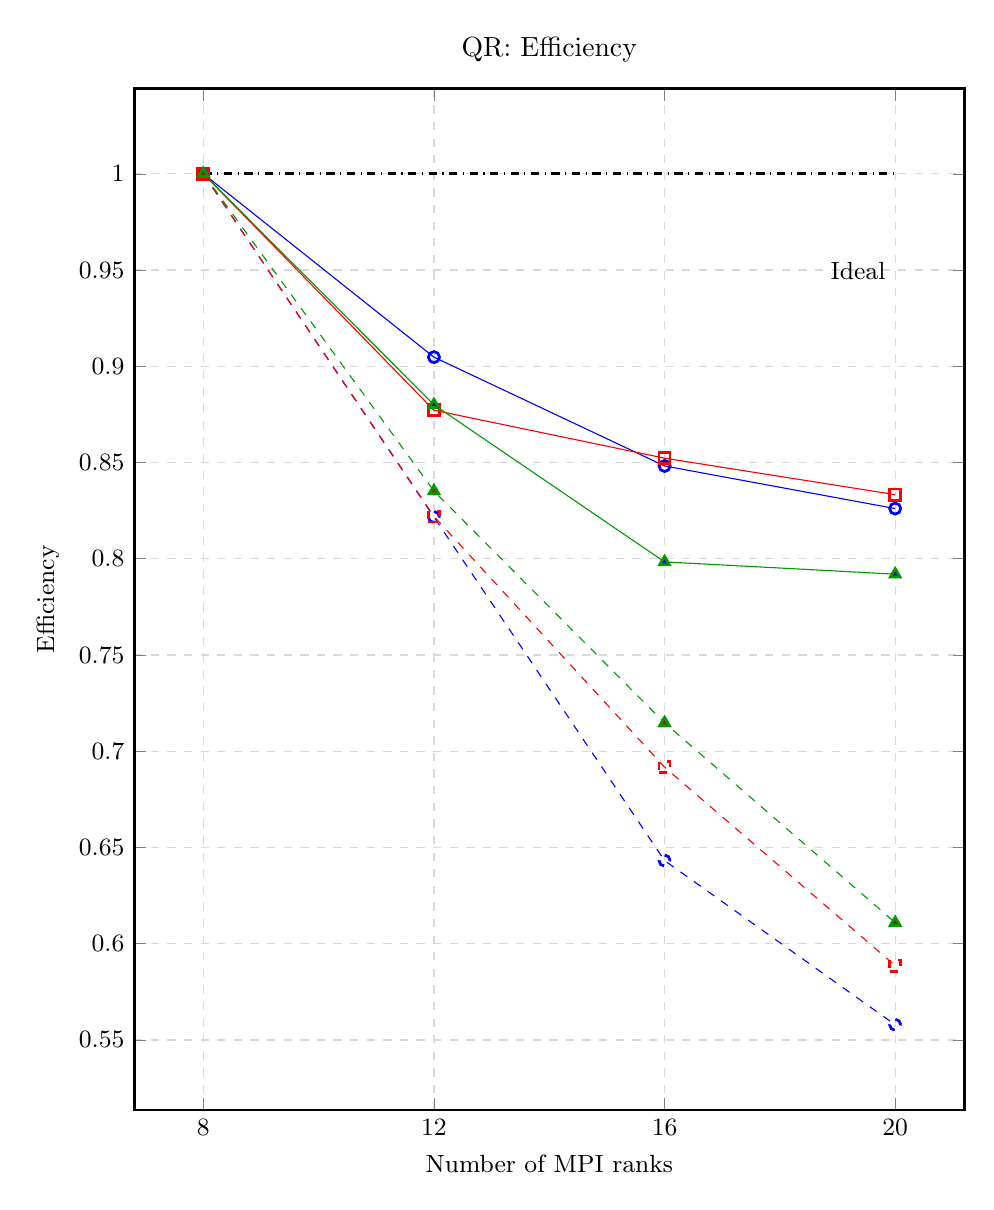
\begin{tikzpicture}
\begin{axis}[
    width=\linewidth,
    height=1.2\linewidth,
    xlabel={Number of MPI ranks},
    ylabel={Efficiency},
    xtick={4,6,8,10},
    xticklabels={8,12,16,20},
    title={QR: Efficiency},
    tick label style={font=\small},
    label style={font=\small},
    grid=major,
    axis line style={black, line width=1pt},
    grid style={dashed, gray!30},
    line width=1pt
]

\addplot+[mark=o, solid, mark size=2pt, blue] coordinates {(4,1.0000) (6,19*4/6/14) (8,19*4/8/11.2) (10,19*4/10/9.2)};
\addplot+[mark=o, dashed, mark size=2pt, blue] coordinates {(4,1.0000) (6,53*4/6/43) (8,53*4/8/41.2) (10,53*4/10/38)};
\addplot+[mark=square, solid, mark size=2pt, red] coordinates {(4,1.0000) (6,75*4/6/57) (8,75*4/8/44) (10,75*4/10/36)};
\addplot+[mark=square, dashed, mark size=2pt, red] coordinates {(4,1.0000) (6,127*4/6/103) (8,127*4/8/91.8) (10,127*4/10/86.3)};
\addplot+[mark=triangle*, solid, mark size=2pt, green!60!black] coordinates {(4,1.0000) (6,198*4/6/150) (8,198*4/8/124) (10,198*4/10/100)};
\addplot+[mark=triangle*, dashed, mark size=2pt, green!60!black] coordinates {(4,1.0000) (6,223*4/6/178) (8,223*4/8/156) (10,223*4/10/146)};
\addplot[
    black,
    dash dot,
    no markers,
    line width=1pt
] coordinates {
    (4,1)
    (6,1)
    (8,1)
    (10,1)
};
\node at (axis cs:10,0.94) [anchor=south east, black, font=\small] {Ideal};
\end{axis}
\end{tikzpicture}
\end{minipage}

% ----------------- Shared legend below all plots -----------------
\vspace{1em}
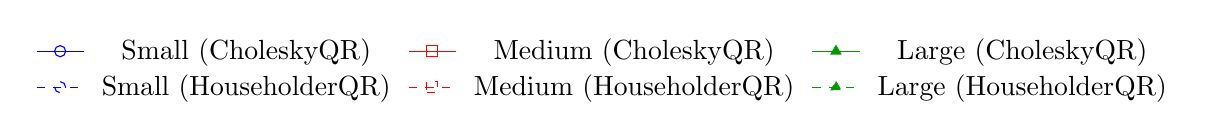
\begin{tikzpicture}
\begin{axis}[
    hide axis,
    xmin=0, xmax=1,
    ymin=0, ymax=1,
    legend columns=3,
    legend style={
        draw=none,
        column sep=1ex
    }
]
% define legend entries without plotting points
\addlegendimage{mark=o, solid, blue}
\addlegendimage{mark=square, solid, red}
\addlegendimage{mark=triangle*, solid, green!60!black}
\addlegendimage{mark=o, dashed, blue}
\addlegendimage{mark=square, dashed, red}
\addlegendimage{mark=triangle*, dashed, green!60!black}

\legend{
Small (CholeskyQR),
Medium (CholeskyQR),
Large (CholeskyQR),
Small (HouseholderQR),
Medium (HouseholderQR),
Large (HouseholderQR)
}
\end{axis}
\end{tikzpicture}

\caption{Strong-scaling performance and parallel efficiency comparison between CholeskyQR and Householder QR across configurations. Each measurement was repeated five times. Runtime plots show the average execution time, with shaded bands indicating the minimum–maximum range across runs. Parallel efficiency is computed from the averaged runtimes.}
\label{fig:combined_strong_scaling}
\end{figure}

The total runtime decreases consistently with increasing MPI process count across all configurations, demonstrating good strong scaling. When CholeskyQR is used, for the smallest case ($\nev+\nex=1800$), the total time drops from approximately $534$s on 16 nodes to $124$s on $100$ nodes. For the largest configuration ($\nev+\nex=6000$), the runtime decreases from about 1890 on $16$ nodes to $702$s on $100$ nodes.
Parallel efficiency relative to the smallest node count declines moderately as expected with increased communication overhead: at $100$ nodes, it ranges from $0.62$-$0.72$ for the smallest configuration to $0.40$-$0.43$ for the largest one. Notice that the parallel efficiency for medium and large $\nev$ degrades more rapidly since both the QR factorization and Rayleigh-Ritz procedure become more relevant overall and do not scale as nicely as the polynomial filter. 

Focusing on the QR factorization, CholeskyQR version consistently outperforms Householder QR across all problem sizes. In the largest configuration ($\nev+\nex=6000$), when executed on $20$ MPI processes within the column communicator, CholeskyQR completes in $100$s compared to $146$s for Householder QR, achieving a speedup of roughly $1.46\times$. For moderate configurations, the speedup even goes up to $2$-$3\times$, and more the smallest case, this speedup can achieve over $4\times$. Since QR is one of the dominant computational components of each ChASE iteration, these reductions in QR time directly contribute to a significant decrease in total runtime, particularly for large eigenproblems.

%\commnt{Edo}{We need to explain why both CholeskyQR and HHQR have a deep in parallel efficiency at 6 nodes count. I also have a question: did you average across all column communicator or did you just pick the first column communicator for the time measurement?} \commnt{XZ}{1. should link to the fact that allreduce used binary-tree scheme. 2. There is always a MPI\_Barrier before mesuring time.}
The parallel efficiency of QR mirrors these improvements. CholeskyQR maintains higher efficiency than Householder QR across all node counts and problem sizes.
For instance, in the largest configuration, CholeskyQR retains an efficiency of about $0.79$-$0.83$ on $8$-$20$ MPI processes in the column communicator, while Householder QR efficiency drops more sharply, to approximately $0.53$–$0.61$. This difference reflects the lower communication overhead and simpler computational structure of CholeskyQR, which allows it to scale more effectively within the column communicator even as the number of nodes increases.

%\commnt{XZ}{I updated all the plots using five repetitions per experiment; running more repetitions would be too time-consuming for some configurations. For the runtime plots, I show the average time with a shaded band indicating the min–max range across the runs (it was somewhat cumbersome to implement this directly in LaTeX). The parallel efficiency is computed using the averaged timings. I also changed the x-axis labels from nodes to MPI ranks. For the QR performed within the column communicator, the relevant measure of parallelism is the number of MPI ranks rather than nodes, since only 2 out of the 4 MPI ranks on each node participate in the QR within a column communicator.} \commnt{Edo}{I think the plot now look quite nice. I also think is a better idea to put MPI ranks since the parallelism is actually explicitly realized on a subset of MPI communicators for QR. Well done! }
Importantly, the convergence behavior of ChASE is essentially unaffected by the choice of QR variants: the total number of iterations and MatVecs remain nearly identical. These results confirm that CholeskyQR variant with heuristic selection can safely replace Householder QR without compromising numerical robustness, while simultaneously delivering higher parallel efficiency, shorter QR execution time, and reduced total time-to-solution.

